\section{Software and Remote Operation}
\label{sec:software}

Once a display is mounted, changing its purpose should be an ordinary task for the people using the room. A teacher preparing an examination needs to set a countdown, office staff need to publish a notice, a maintainer needs to update the firmware. The software supports these activities through a device-hosted configuration page and a remote web dashboard, while the microcontroller handles the displayed content and timing.

\subsection{Connecting an Installed Display}

Network setup begins at the display itself. Holding the local button activates AP mode, allowing a phone to connect directly to the device. The user then opens the device's IP address in a browser, scans nearby Wi-Fi networks, and supplies the required credentials. The portal lists networks by signal strength and identifies saved entries. Up to five network profiles are retained in flash, allowing credentials to survive a restart.

The configuration page and its HTTP server are implemented within the Zephyr application. This gives the device a setup interface before it has access to the dashboard or external network services. After provisioning, the user can reconnect the phone to its normal network and open the dashboard in the same browser. No dedicated mobile application or programming cable is required.

\subsection{Changing the Display's Role}

The dashboard provides controls for clockface selection, notices, and timers. Figure~\ref{fig:dashboard} shows two common tasks. For a timer, the user chooses a duration, selects count-up or countdown operation, and requests an immediate or scheduled start. The interface also lists scheduled activities with their start and end times. For a notice, the user enters the message and selects its display duration or date-and-time interval.

\begin{figure*}[t]
\centering
\begin{minipage}[b]{0.49\textwidth}
\centering
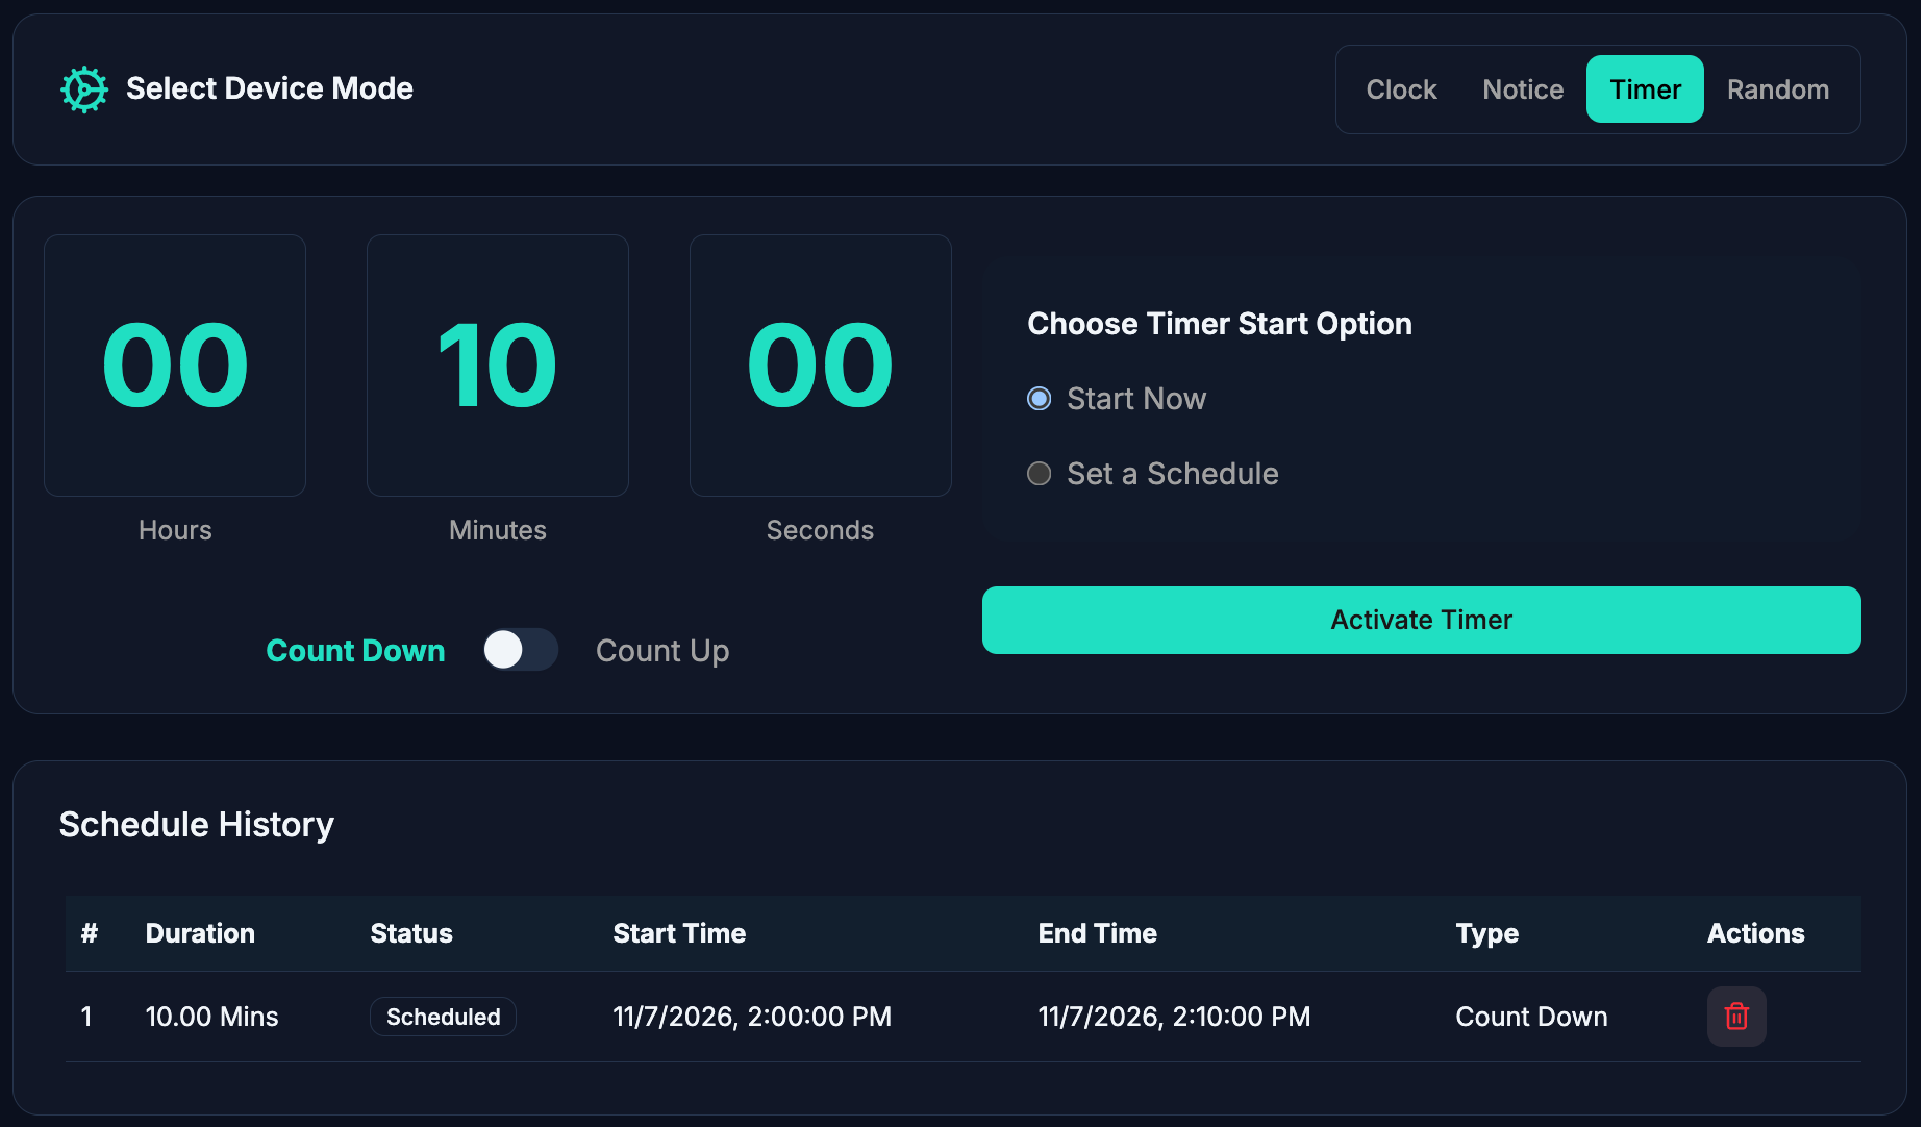
\includegraphics[width=\linewidth]{figs/dashboard_timer}
\par\vspace{2pt}
{\footnotesize (a) Timer control}
\end{minipage}
\hfill
\begin{minipage}[b]{0.49\textwidth}
\centering
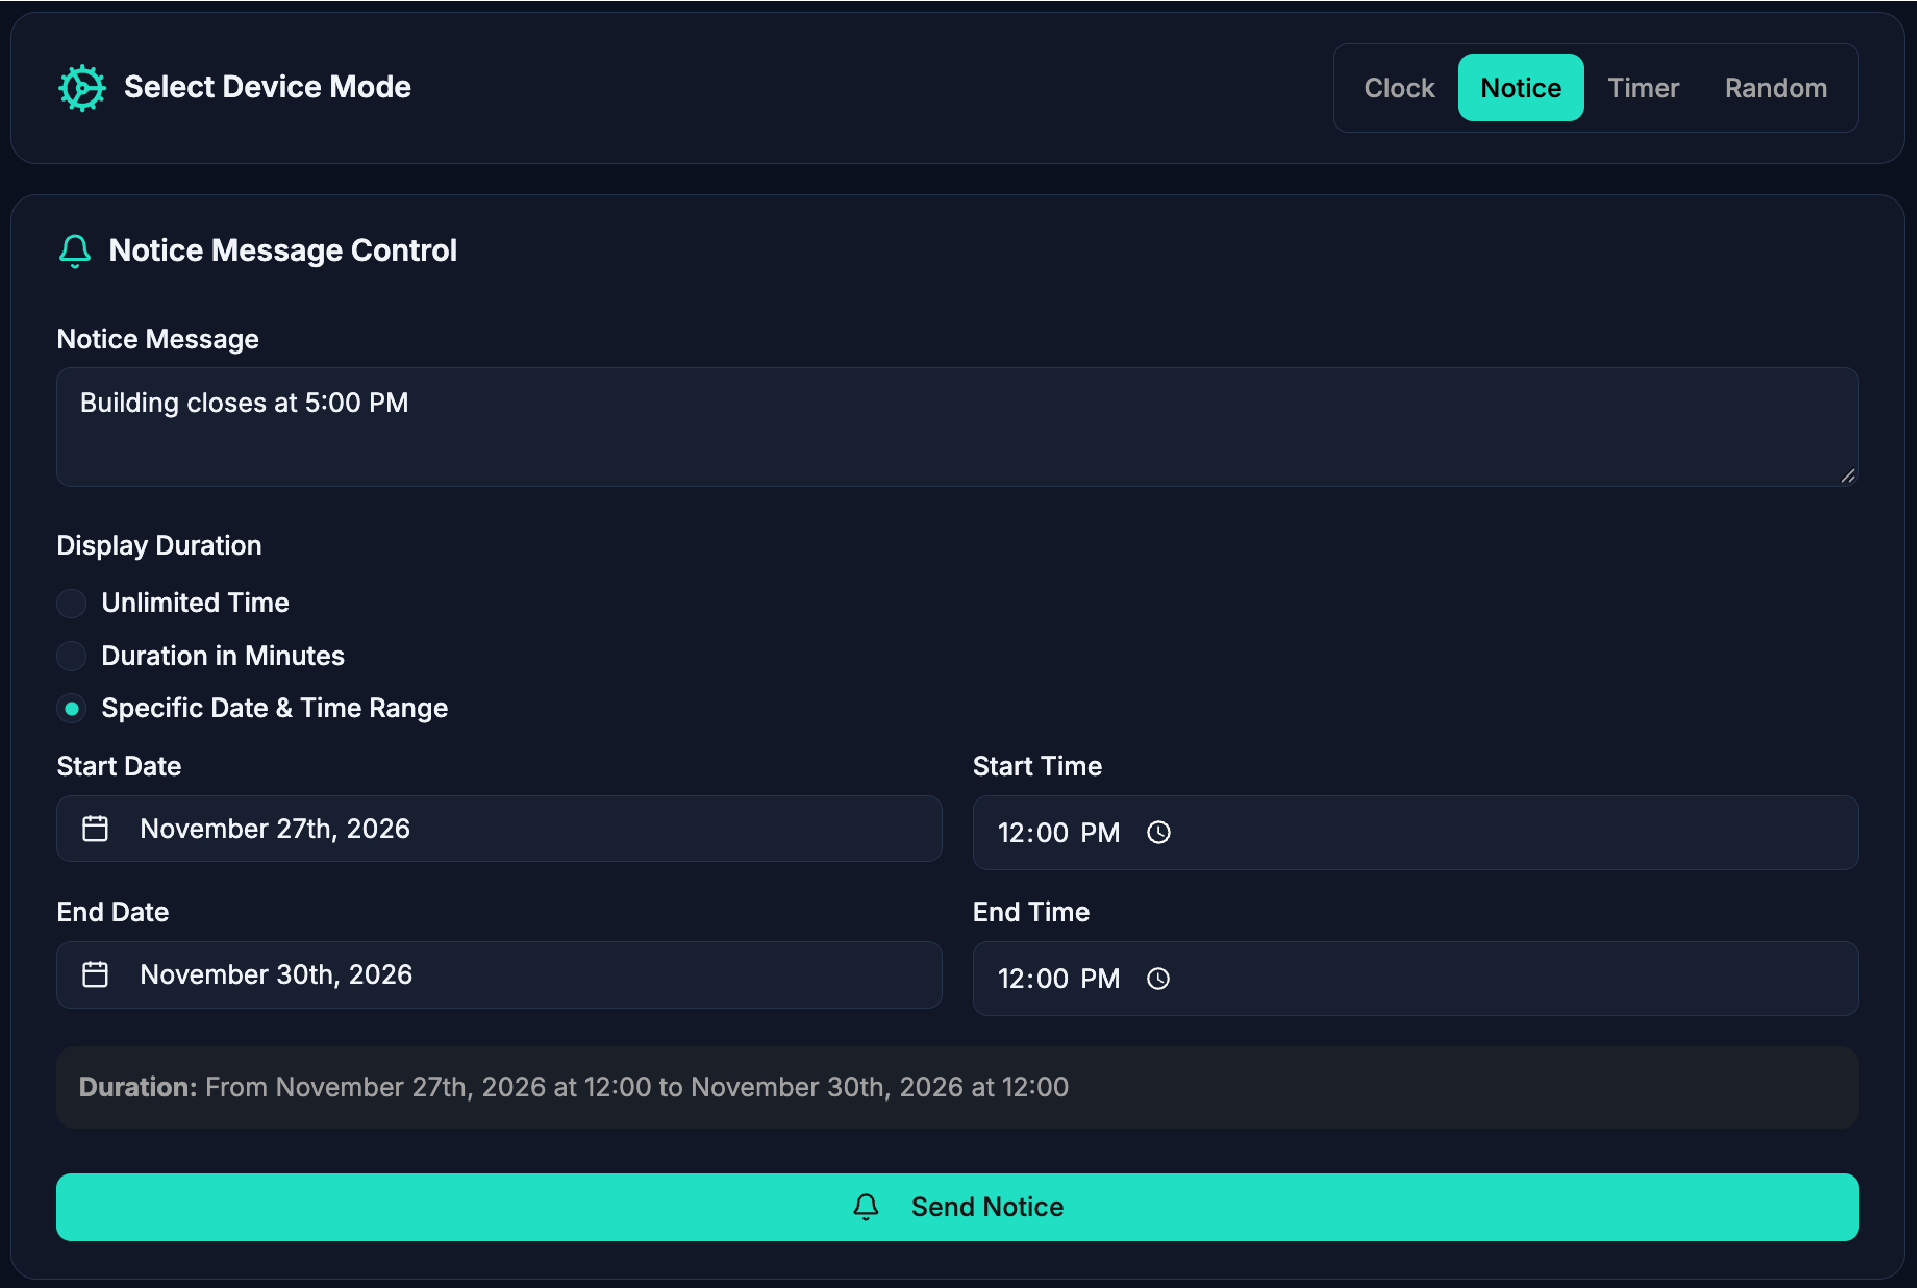
\includegraphics[width=\linewidth]{figs/dashboard_notice}
\par\vspace{2pt}
{\footnotesize (b) Notice scheduling}
\end{minipage}
\caption{Web dashboard interfaces for (a) configuring timers and viewing scheduled activities and (b) composing notices with a specified display interval.}
\label{fig:dashboard}
\end{figure*}

MQTT carries commands to the selected device, which generates the displayed content locally. Users can change clockfaces, publish notices, and configure timed activities through the dashboard. The dashboard also exposes device status, the reported operating mode, and firmware version, helping users identify the unit they are managing.

\subsection{Keeping Display Operation Responsive}

Network activity and display rendering have different rhythms. A connection attempt may take seconds, while scrolling text needs frequent updates. The application therefore handles Wi-Fi connection management and MQTT processing separately from the display thread. Network connection attempts proceed in the background, and the display thread renders the current mode into a shared framebuffer.

The application retains settings such as the selected clockface, notice text, brightness, and timer timestamps. These saved values support restoration after a restart, including the schedule recovery described in the \nameref{sec:system_overview} section. Network time synchronization updates the RTC when connectivity is available.

\subsection{Updating Firmware After Installation}

Firmware maintenance follows a similar remote workflow. An update command supplies the firmware image URL, and the device downloads the image into a secondary flash slot. During the transfer, the LED panels show update progress, giving someone near the display a visible explanation for the interruption to normal operation. Progress and error messages are also published over MQTT.

After staging the image, the application requests an MCUboot test upgrade and restarts. MCUboot validates the image signature before allowing the new firmware to run. This permits software changes after installation while checking that the replacement image was signed with the expected key.